% Appendix A

\chapter{Introduction to Quantum Computing} % Main appendix title
This appendix serves as a quick introduction to quantum computing. We explain the basics concepts without going deeply into their physical meaning or historical approach. For a deeper discussion of the topics described herein, we refer the reader to Refs. \cite{W.Bryon1992HilbertFunctions},  \cite{Scherer2019MathematicsComputing} and \cite{Nielsen2010QuantumInformation}.
\label{AppendixA} % For referencing this appendix elsewhere, use \ref{AppendixA}
%%%%%%%%%%%%%%%%%%%%%%%%%%%%%%%%%%%%%%%%%%%%%%%%%%%%%%%%%%%%%%%%%%%%%%%%%%%%%%%%%%%%%%%%%%%%%%%%%%%%%%%%%%
%     A.1 HILBERT SPACE
%%%%%%%%%%%%%%%%%%%%%%%%%%%%%%%%%%%%%%%%%%%%%%%%%%%%%%%%%%%%%%%%%%%%%%%%%%%%%%%%%%%%%%%%%%%%%%%%%%%%%%%%%%
\section{Hilbert space}
We start by defining the vector space where quantum computing takes place, the Hilbert space, $\mathbb{H}$.
\begin{definition}[Hilbert Space]
A Hilbert space is a special type of linear vector space whose elements are complex-valued \textit{square integrable}\footnote{A function $\psi(x)$ is said to be \textit{square integrable} on a given interval $\left[a, b\right]$ if $\int_{a}^{b}\|\psi(x)\|^{2}dx$ exist with a finite value.} functions, $\psi(x)$, of a real variable $x$, defined on the closed interval $\left[a, b\right]$, equipped with a \textit{complete inner product}, $(\cdot,\cdot)$, in $\mathbb{C}$.
\end{definition}
\begin{definition}[Inner Product]
Given two functions of the Hilbert space, $\psi_{1}$ and $\psi_{2}$, the inner product is defined by
\begin{equation}
    \left(\psi_{1}, \psi_{2}\right) \equiv \int^{b}_{a} \psi_{1}^{*}(x)\psi_{2}(x)dx
\end{equation}
\end{definition}
\begin{corollary}
Given the functions \{$\psi_{1}$,$\psi_{2}$,$\psi_{3}$\} $\in \mathbb{H}$ and \{$\alpha, \beta\} \in \mathbb{C}$, the inner product of the associated Hilbert space satisfies:
\begin{itemize}
    \item Closed operation: $(\psi_{1},\psi_{2})\in \mathbb{C}$
    \item Conjugate symmetry: $(\psi_{1},\psi_{2}) = (\psi_{2},\psi_{1})^{*}$
    \item Linear with respect to the second vector: $(\psi_{1},\lambda \cdot \psi_{2} + \beta\cdot\psi_{3}) = \lambda(\psi_{1},\psi_{2}) + \beta(\psi_{1},\psi_{3})$
    \item Anti-linear with respect to the first vector: $(\lambda \cdot \psi_{1} + \beta \cdot \psi_{2}, \psi_{3}) = \lambda^{*}(\psi_{1},\psi_{3}) + \beta^{*} (\psi_{2},\psi_{3})$
    \item Positive definiteness: $(\psi, \psi) = \lVert \psi \rVert^{2} \in \left[0,\infty\right)$\footnote{The quantity $\lVert \psi \rVert^{2}$ is called the norm of $\psi$. If $\lVert \psi \rVert^{2} = 0$ that does not imply $\psi(x) = 0$ for all $x$ in $\left[a,b\right]$. The function can have nonzero values at some points and the integral will remain zero. The integral roughly computes the area in a given interval, so, if there is just a point not null in the interval the area captured by a point is zero, so its contributions to the integral is zero. In our case the quantity $\lVert \psi \rVert^{2}$ represents the probability density of a given state $\psi$, i.e., if we integrate the whole interval of definition $x \in D$, $\int_{D}\lVert \psi \rVert^{2}dx = 1$.} 
\end{itemize}    
\end{corollary}
\begin{definition}[Distance]
    The distance defined by Hilbert space's inner product is given by
    \begin{equation}
      d \equiv \left|\psi_{2} - \psi_{1}\right| = \sqrt{(\psi_{2}-\psi_{1},\psi_{2}-\psi_{1})}  
    \end{equation}
\end{definition}
\begin{definition}[Completeness of a space]
A complete space is one in which any Cauchy sequence -- of that space -- is convergent, i.e., tends towards a value inside the given space.
\end{definition}
We can show why completeness of space is a necessary condition. Suppose that our space is not complete, i.e., some Cauchy sequences are not convergent. Then, the evolution of an initial state\footnote{The formulae for the evolution of n state is explained in later sections.}, $\ket{\psi(0)}$, under a given constant Hamiltonian is not guaranteed\footnote{It is not guaranteed that the Cauchy sequence $\sum_{i = 0}^{n}(-it)^{k} / \left(k!h^{k}\right)\mathcal{H}^{k}$ converges.}
\begin{equation}
    \ket{\psi(t)} = e^{-\frac{i\mathcal{H}}{\hbar}t}\ket{\psi(0)} = \lim_{n \to \infty} \sum_{i = 0}^{n}\frac{(-it)^{k}}{k!h^{k}}\mathcal{H}^{k}\ket{\psi(0)}
\end{equation}
\begin{definition}[Completeness of an orthonormal set of functions]
A set of orthonormal functions $\{\psi_{i}\}$ is complete if any function $\psi(x)$ in Hilbert space can be written as a linear combination of the $\psi_{i}(x)$\footnote{Here we do not ask for point convergence, we weaken the converge criteria to mean convergence. Otherwise, there would not exist a complete set of orthonormal function in the Hilbert space.}:
\begin{equation}
    \lim_{n\to \infty}\| \psi(x) - \sum_{i=1}^{n}c_{i}\psi_{i}(x)\|^{2} = 0
\end{equation}
\end{definition}
\begin{theorem}[Riesz-Fischer]
Assume the functions $\psi_{1}(x),\psi_{2}(x),\ldots$ are elements of Hilbert space. If
\begin{equation}
    \lim_{n,m\to\infty} \lVert \psi_{n} - \psi_{m}\rVert^{2} \equiv \lim_{n,m\to \infty} \int_{a}^{b} \|\psi_{n} - \psi_{m}\|^{2}dx = 0
\end{equation}
then there exist a square (Lebesgue) integrable function $\psi(x)$ to which the sequence $\psi_{n}(x)$ converges such that 
\begin{equation}
    \lim_{n\to \infty} \int_{a}^{b} \|\psi - \psi_{n}\|^{2}dx = 0
\end{equation}
Equivalently, let $\psi_{n}$ be a Cauchy sequence and $\psi$ a value inside the given space. Then, the Cauchy sequence converges to $\psi(x)$ \textit{in the mean}, i.e, we allow the difference $\|\psi(x) - \psi_{n}(x)\|^{2}\neq 0$ at some points $x$, so that the integral $\lim_{n\to \infty} \int_{a}^{b} \|\psi - \psi_{n}\|^{2}dx$ is zero when taking into account the whole interval.
\end{theorem}
\begin{definition}[Orthonormality]
A given set of functions $\{\psi_{i}\}$ is said to be orthonormal if
\begin{equation}
    \left(\psi_{i}, \psi_{j}\right) \equiv \int_{a}^{b} \psi_{i}^{*}(x)\psi_{j}(x) dx = \delta_{ij} 
\end{equation}
\end{definition}
In the present work we work with a particular Hilbert space, a finite Hilbert space. This implies our space is \textit{separable}.
\begin{definition}[Separable]
    A Hilbert space is said to be \textit{separable} if an only if it has a countable orthonormal basis.
\end{definition}
So for a finite Hilbert space -- which is a countable space -- an orthogonal basis is guaranteed.
%%%%%%%%%%%%%%%%%%%%%%%%%%%%%%%%%%%%%%%%%%%%%%%%%%%%%%%%%%%%%%%%%%%%%%%%%%%%%%%%%%%%%%%%%%%%%%%%%%%%%%%%%%
%     A.2 NOTACION
%%%%%%%%%%%%%%%%%%%%%%%%%%%%%%%%%%%%%%%%%%%%%%%%%%%%%%%%%%%%%%%%%%%%%%%%%%%%%%%%%%%%%%%%%%%%%%%%%%%%%%%%%%
\section{Notation}
\begin{definition}[Dirac's Bra-Ket Notation]
The inner product of an n-dimensional Hilbert space defines a linear map from $\mathbb{H}$ to $\mathbb{C}$
\begin{align*}
  \tau: \mathbb{H}\longrightarrow& \mathbb{C}^{n} \\
  \tau(\psi) \longrightarrow& \begin{bmatrix}
           \alpha_{1} \\
           \vdots \\
           \alpha_{n}
         \end{bmatrix}
\end{align*}  
Conversely, 
\begin{align*}
  \bar{\tau}: \mathbb{H}^{*}\longrightarrow& \mathbb{C}^{n} \\
  \bar{\tau}(\psi)\longrightarrow& 
         \begin{bmatrix}
           \alpha_{1}^{*}, \hdots, \alpha_{n}^{*}
         \end{bmatrix}
\end{align*} 
where $\mathbb{H}^{*}$ denotes the dual space. The dual space $\mathbb{H}^{*}$ is also a Hilbert space with the same dimension as $\mathbb{H}$. 
\begin{itemize}
    \item Elements of a Hilbert space, $\mathbb{H}$ are called \textit{ket-vectors} 
\begin{equation}
    \psi \equiv \ket{\psi} =  \begin{bmatrix}
           \alpha_{1} \\
           \vdots \\
           \alpha_{n}
         \end{bmatrix}
\end{equation}
\item Elements of a dual Hilbert space $\mathbb{H}^{*}$ are called \textit{bra-vectors}
\begin{equation}
    \psi^{*} \equiv \bra{\psi} =  \begin{bmatrix}
           \alpha_{1}^{*}, & \hdots &, \alpha_{n}^{*}
         \end{bmatrix}
\end{equation}
\end{itemize}
\end{definition}

Notice that a bra-vector is just the transpose conjugate of a ket-vector. This is a useful way of mapping a ket-vector of a given Hilbert space into its bra-vector on the associated dual Hilbert space.

\begin{corollary}
    In bra-ket notation, a set of vectors $\{\ket{\psi_{j}}\}$ is said to span $\mathbb{H}$ if we can express any vector $\ket{\psi}$ of that space as a linear combination of the vectors in the given set
    \begin{equation}
        \ket{\psi} = \sum_{j}\alpha_{j}\ket{\psi_{j}}
    \end{equation}
    where the coefficients of the combination $\alpha_{j}$ are complex numbers. In particular, if the set of vectors $\{\ket{\psi_{j}}\}$ are linearly independent and the number of vectors in that set is equal to the dimension of our space, then this set of vectors is a basis set of our space and the previous expression is the so-called basis expansion of $\ket{\psi}$.
\end{corollary}
%%%%%%%%%%%%%%%%%%%%%%%%%%%%%%%%%%%%%%%%%%%%%%%%%%%%%%%%%%%%%%%%%%%%%%%%%%%%%%%%%%%%%%%%%%%%%%%%%%%%%%%%%%
%     A.3 Quantum bits
%%%%%%%%%%%%%%%%%%%%%%%%%%%%%%%%%%%%%%%%%%%%%%%%%%%%%%%%%%%%%%%%%%%%%%%%%%%%%%%%%%%%%%%%%%%%%%%%%%%%%%%%%%
\section{Quantum bits}
A \textit{bit} is the smallest unit of information of classical computing. Analogously, a \textit{qubit} is the smallest unit of information for quantum computing. The following section treats bits and qubits as abstract mathematical objects without their physical implementation. In Appx.\,\ref{AppendixC}, we describe some implementations of a physical qubit.\\\\
A classical bit has two possibles states commonly named $\ket{0}$ or $\ket{1}$\footnote{The name of the states of a bit or qubit is not important. It is just a way of labelling those states.}. However, a quantum bit is a linear combination of states -- \textit{superposition} -- $\{\ket{0}, \ket{1}\}$. The general state of a qubit can be conceived as a vector in a two-dimensional complex vector space, with $\alpha, \beta \in \mathbb{C}$
\begin{equation}
    \ket{\psi} = \alpha \ket{0} + \beta \ket{1} = \alpha \begin{bmatrix}
           1 \\
           0 
         \end{bmatrix}
         +
         \beta
         \begin{bmatrix}
           0 \\
           1 
         \end{bmatrix}
\end{equation}
where $\|\alpha\|^{2} + \|\beta\|^{2}$ = 1, i.e, the state of a qubit is normalized.\\
The last expression can be written in term of two parameters,
\begin{equation}
    \ket{\psi} = \cos{\frac{\theta}{2}}\ket{0} + e^{i\phi}\sin{\frac{\theta}{2}}\ket{1}
\end{equation}
that represent the angles of the Bloch Sphere\footnote{A Bloch sphere is a geometric representation of the state of a single qubit where each axis has two orthogonal states, e.g., the Z-axis has the orthogonal states $\{\ket{0},\ket{1}\}$.}.\\
The states $\ket{0}$ and $\ket{1}$ form a computational basis (orthonormal basis) for the $\mathbb{C}^{2}$ vector space. There are infinite single-qubit basis sets for $\mathbb{C}^{2}$, albeit the ones known as \textit{computational basis} are the ones that build the axis of the Bloch Sphere.

\begin{figure}[h]
    \centering
    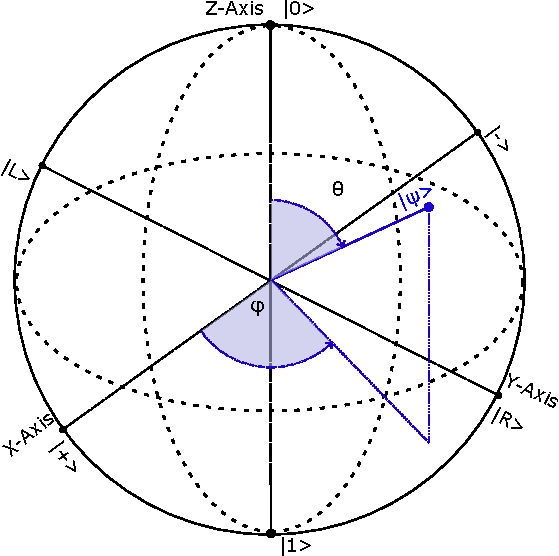
\includegraphics[scale=0.8]{Figures/BlochSphere.pdf}
    \caption{A Bloch Sphere displaying the state $\ket{\psi}$ of a single qubit.}
    \label{fig:bloch_sphere}
\end{figure}
The Pauli matrices represent a rotation\footnote{Pauli matrices are generators of SU(2) group. A complex exponential can be understood as a rotation around a vector $\vec{n}$ where $e^{i\frac{\theta}{2}(\vec{n}\cdot \vec{\sigma})} = \mathbb{I}\cos{\frac{\theta}{2}} + i(\vec{n}\cdot \vec{\sigma})\sin{\frac{\theta}{2}}$.} around a given axis $\{X, Y, Z \}$. The matrix representation is given by,
\begin{align*}
X \equiv \sigma_{x} = \sigma_{1} = 
    \begin{bmatrix}
           0 & 1 \\
           1 & 0 
         \end{bmatrix} \\
Y \equiv \sigma_{y} = \sigma_{2} = 
    \begin{bmatrix}
           0 & -i \\
           i & 0 
         \end{bmatrix} \\ 
Z \equiv \sigma_{z} = \sigma_{3} = 
    \begin{bmatrix}
           1 & 0 \\
           0 & -1 
         \end{bmatrix}
\end{align*}
The eigenvectors of the Pauli matrices are the computational basis vectors,
\begin{align*}
    \Biggl\{\begin{bmatrix}
           1 \\
           0 
         \end{bmatrix}, \begin{bmatrix}
           0 \\
           1 
         \end{bmatrix} \Biggr\}\equiv \{\ket{0}, \ket{1}\} \in Z_{basis} \\
         \Biggl\{\begin{bmatrix}
           \frac{1}{\sqrt{2}} \\
           \frac{1}{\sqrt{2}} 
         \end{bmatrix}, \begin{bmatrix}
           \frac{1}{\sqrt{2}} \\
           -\frac{1}{\sqrt{2}} 
         \end{bmatrix} \Biggr\}\equiv \{\ket{+}, \ket{-}\} \in X_{basis} \\
         \Biggl\{\begin{bmatrix}
           \frac{1}{\sqrt{2}} \\
           \frac{i}{\sqrt{2}} 
         \end{bmatrix}, \begin{bmatrix}
           \frac{1}{\sqrt{2}} \\
           -\frac{i}{\sqrt{2}} 
         \end{bmatrix} \Biggr\}\equiv \{\ket{R}, \ket{L}\} \in Y_{basis}
\end{align*}
In general, we deal with multiple qubits. The basis for an n-qubit system is just the tensor product of n-single-qubit basis.\\
Suppose we have two qubits. Then, the $Z\otimes Z-basis$ is $\{\ket{00},\ket{01},\ket{10},\ket{11}\}$ and the state of a two-qubit system is described by the linear combination,
\begin{equation}
    \ket{\psi} = \alpha_{00}\ket{00} +\alpha_{01}\ket{01} +\alpha_{10}\ket{10} +\alpha_{11}\ket{11}
\end{equation}
where $\|\alpha_{00}\|^{2} + \|\alpha_{01}\|^{2} + \|\alpha_{10}\|^{2} + \|\alpha_{11}\|^{2} = 1$, i.e., the state is normalized.\\
The normalization condition for an n-qubit system can be written as
\begin{equation}
\sum_{x\in \{0,1\}^{n}}\|\alpha_{x}\|^{2} = 1
\end{equation}
Where the expression $x \in \{0,1\}^{n}$ indicates all the possible tensor product combinations of the n-single-qubit states. These combinations form a basis for the n-qubit system.
%%%%%%%%%%%%%%%%%%%%%%%%%%%%%%%%%%%%%%%%%%%%%%%%%%%%%%%%%%%%%%%%%%%%%%%%%%%%%%%%%%%%%%%%%%%%%%%%%%%%%%%%%%
%     A.4 MEASUREMENTS AND OPERATORS
%%%%%%%%%%%%%%%%%%%%%%%%%%%%%%%%%%%%%%%%%%%%%%%%%%%%%%%%%%%%%%%%%%%%%%%%%%%%%%%%%%%%%%%%%%%%%%%%%%%%%%%%%%
\section{Measurements and Operators}
Quantum mechanics makes predictions about microscopic objects taking into account their statistics\footnote{Measurements in an ensemble of equally prepared states gives quantities distributed around a mean value with a given frequency.}. The predictions have implications for the macroscopic world. In classical computing a system is mostly unaltered by tiny interactions such as light or heat. However, in quantum computing this environment noise is quite important as it modify the state of the system. This noise is a doubled-edged sword as it can be used to modify intentionally the state of a quantum system.
\begin{definition}[Operator]
    An operator $\hat{A}$ is a linear map between Hilbert spaces that satisfy,
    \begin{equation}
        \braket{\hat{A}^{\dagger}\psi|\varphi} = \braket{\psi|\hat{A}\varphi} \forall \psi,\varphi \in \mathbb{H}
    \end{equation}
    where $\hat{A}$ admit a matrix representation and "$\dagger$" means transpose conjugate
\end{definition}
\begin{corollary}
    Given an operator $\hat{A}$, on a finite Hilbert space, the operator is said to be Hermitian if
    \begin{equation}
        \hat{A}^{\dagger} = \hat{A}
    \end{equation}
    Hermitian operators play an important role in quantum physics because their eigenvalues are real and represent measurable physical quantities.
\end{corollary}
\begin{definition}[Observable]
    Given the state of a system $\ket{\psi}$, an \textit{observable} -- represented with an operator $\hat{A}$ -- is the physical quantity we can measure associated with the Hermitian operator $\hat{A}$. The possible observables of an operator are its eigenvalues.
\end{definition}
As an example consider the \textit{Hamiltonian} of a system, $\hat{\mathcal{H}}$. For the present work, the Hamiltonian of a system represents the total energy of the system. So, the associated eigenvalues are the eigenenergies of the system.  
\begin{definition}[Unitary Operator]
    An operator U on $\mathbb{H}$ is unitary if
    \begin{equation}
        U^{\dagger}U =\mathbb{I}
    \end{equation}
where $\mathbb{I}$ is the identity operator.
\end{definition}
\begin{definition}[Expectation Value]
    The expectation value, $<\cdot>$, of an observable is the mean value we get after a sequence of measurements of that observable in an ensemble of equally prepared states.
        Mathematically,
    \begin{equation}
        \langle\hat{A}\rangle_{\ket{\psi}} := \braket{\psi |\hat{A}| \psi}
    \end{equation}
\end{definition}

We can measure a classical bit to check if it is in the state 0 or 1. However, when we measure -- in the Z-basis -- a quantum bit we do not get the parameters $\alpha, \beta$ that describe the qubit state. Instead, we get either $\ket{0}$ or $\ket{1}$ with probabilities $\|\alpha\|^{2}$ and $\|\beta\|^{2}$ respectively. The logic of classical computing is Boolean, this means that if the system is not in the state 0 it must be in state 1. In quantum computing, if the system is not in the state 0 it does not have to be in state 1.   

In a measurement, the general state of the qubit collapses to one of the states of the basis we are using to measure. After this measurement the state of our qubit is fixed and successive measurements will give the same state with probability 1, i.e., measurements collapse a qubit into one of the basis states destroying superposition. Quoting Nielsen and Chuang\,\cite{Nielsen2010QuantumInformation},
\begin{displayquote}
\textit{This dichotomy between the unobservable state of a qubit and the observations we can make lies at the heart of quantum computation and quantum information.}
\end{displayquote}
%%%%%%%%%%%%%%%%%%%%%%%%%%%%%%%%%%%%%%%%%%%%%%%%%%%%%%%%%%%%%%%%%%%%%%%%%%%%%%%%%%%%%%%%%%%%%%%%%%%%%%%%%%
%     A.5 SCHRODINGER EQUATION
%%%%%%%%%%%%%%%%%%%%%%%%%%%%%%%%%%%%%%%%%%%%%%%%%%%%%%%%%%%%%%%%%%%%%%%%%%%%%%%%%%%%%%%%%%%%%%%%%%%%%%%%%%
\section{Schrödinger Equation}
One of the paradigms of universal quantum computing is the gate model. This approach substitutes classical logic gates -- such as OR, XOR, AND or NOT -- by its quantum analog. These quantum gates are represented by unitary matrices, so that the inner product is preserved.\\
Equivalently, a quantum gate is represented by a complex exponential of the form\footnote{Where $\hbar$ is the reduced Planck constant.} $\exp\left(i\hat{\mathcal{H}}t / \hbar\right)$ where a given Hamiltonian, $\mathcal{H}$ -- controlled by external fields such as magnetic fields -- leads the evolution of the qubit in such a way that the associated matrix of the complex exponential -- that admit a series expansion -- match the matrix representation of the quantum gate. \\\\
Precisely, the evolution of a quantum system is goberned by the Schrödinger equation which cannot be derived from first principles, i.e., it is an experimental fact. Mathematically, it can be expressed as
\begin{equation}
    \hat{\mathcal{H}}\ket{\psi(t)} = i\hbar \frac{\partial}{\partial t}\ket{\psi(t)}
\end{equation}
where $\hat{\mathcal{H}}$ is the Hamiltonian operator, $\hbar$ is the reduced Planck constant and $\ket{\psi(t)}$ represents the state of a system.\footnote{Remember that in Quantum Physics time does not have an operator so it is not an observable.} and $\ket{\psi(t)}$ represent the state of a system.\\
The Schrödinger equation governs the time evolution of a quantum system. It plays the same role that Newton's equations do in classical mechanics.
%%%%%%%%%%%%%%%%%%%%%%%%%%%%%%%%%%%%%%%%%%%%%%%%%%%%%%%%%%%%%%%%%%%%%%%%%%%%%%%%%%%%%%%%%%%%%%%%%%%%%%%%%%
%     A.6 SPEED-UP ADVANTAGE
%%%%%%%%%%%%%%%%%%%%%%%%%%%%%%%%%%%%%%%%%%%%%%%%%%%%%%%%%%%%%%%%%%%%%%%%%%%%%%%%%%%%%%%%%%%%%%%%%%%%%%%%%%
\section{Speed-up advantage}
We end up this appendix by discussing the main features of quantum behavior that speed-up the algorithms versus its classical approach.\\\\
The main power of quantum computers underlies in three properties,
\begin{itemize}
    \item \textbf{Superposition:} A qubit can be a in a linear combination of states. We can build quantum algorithms that cross out those terms that are not interesting for us and increase the amplitudes of the ones we are interested in.
    \item \textbf{Entanglement:} An entangled state is a state that cannot be written in term of the tensor product of pure states. Entangled states store information exponentially instead of linearly (as classical computing does). As an example, suppose we have the following two-qubit state, called \textit{Bell state}
\begin{equation}
    \ket{\psi} = \frac{1}{\sqrt{2}}\left(\ket{00} + \ket{11}\right)
\end{equation}
If we measure the first qubit in the Z-basis, we can get either the state $\ket{0}$ or $\ket{1}$. We can see that both qubits are entangled in the sense that knowing the state of the first qubit allows us to determine the state of the second qubit. In this case, if the first qubit measurement is $\ket{0}$ we know that the second qubit must be in state $\ket{0}$.\footnote{Einstein termed this effect \emph{spooky action at a distance} in an attempt to ridicule quantum mechanics.}  
    \item \textbf{Parallelism:} A quantum memory register can exist in a superposition of states. If we perform an operation on this quantum register, this operation is applied to all states of that superposition. Notice that we have applied an operation to all the states in that superposition by performing the function just once.
\end{itemize}
Despite the advantage of using quantum computing with respect to classical computing has been proven theorically for some specific problems, see Ref. \cite{Grover19961996Search}, the real world problems are yet far away from being addressed fully by quantum computing\footnote{Nowadays, the hardware is not mature enough for real world industry problems.}. The best we can do nowadays is to solve problems by splitting them into a quantum part that can be done by a quantum computer and a classical part that is solved by using an HPC.
%%%%%%%%%%%%%%%%%%%%%%%%%%%%%%%%%%%%%%%%%%%%%%%%%%%%%%%%%%%%%%%%%%%%%%%%%%%%%%%%%%%%%%%%%%%%%%%%%%%%%%%%%%
%     A.6.1 Grover's Algorithm
%%%%%%%%%%%%%%%%%%%%%%%%%%%%%%%%%%%%%%%%%%%%%%%%%%%%%%%%%%%%%%%%%%%%%%%%%%%%%%%%%%%%%%%%%%%%%%%%%%%%%%%%%%
\subsection{Grover's Algorithm}
In this section we show the advantages of quantum computing by considering a specific example, that of Grover's algorithm.\\
Grover's algorithm is a search algorithm that uses qubits in superposition adjusting their phases to make the computations by quantum parallelism. Given a table with a number of items \textit{N}, we are interested in a particular item $\omega$. The best known classical algorithm can solve the problem in $O(N)$ complexity, which means that in the worst case a classical algorithm has to check each entry of the data-set until finding the item $\omega$ in the last query. Grover's algorithm can solve the problem in $\sim$ $O(\sqrt{N})$ complexity\footnote{This is a lower bound but in some cases the speed up could be better as it happens with the two-qubit system.}, which represent a quadratic speed up compared with the classical approach, i.e., after $\sqrt{N}$ evaluations it is guaranteed to provide the desired state.
\begin{figure}[h]
    \centering
    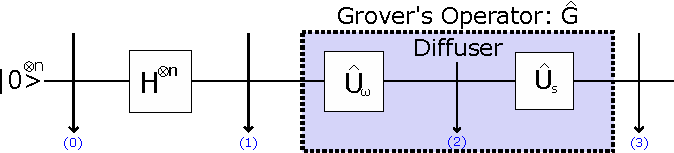
\includegraphics[width=\textwidth]{Figures/Grover_Circuit.pdf}
    \caption{Circuit scheme of Grover's algorithm for an n-qubit system.}
    \label{fig:Grover_circuit}
\end{figure}
\subsubsection{Grover's Algorithm steps for a two-qubit system ($N=4$)}
In this section we show what is the state of the system at each step -- after the application of the quantum gates -- and a geometrical representation based on Ref. \cite{Lavor2008Search} and \textbf{REF}.\\
As an example consider the following table,
\begin{table}[h]
\label{tab:GroverSearch}
\centering
\begin{tabular}{ c | c | c | c | c }
  \hline			
  Binary Index & 00 & 01 & 10 & 11 \\
    \hline		
  Item & 0 & 1 & 2 & 3 \\
  \hline  
\end{tabular}
\caption{Different items described by its binary expansion.}
\end{table}
and suppose we want to find the item 2, where the index -- binary expansion of decimal index starting from zero -- represents the eigenstate of the system we are looking for. Then, if we are interested in finding the item 2, we are looking for the eigenstate $\ket{\omega} = \ket{10}$.\\
\textbf{(0). Initialized single qubit states:} All the qubits are initialized at $\ket{0}$ so the state of the system is given by the tensor product of the qubits,
\begin{equation}
    \ket{\psi_{0}} = \ket{0}\otimes \ket{0} = \ket{00}
\end{equation}
\textbf{(1). Equiprobability:} Apply a Hadamard gate to each qubit so we create a configuration of equiprobable states\footnote{At the beginning we do not have a good guess of where the item can be so each possibility is equally probable.},
\begin{equation}
    \ket{\psi_{1}} = \hat{H}^{\otimes 2}\ket{00} = \frac{1}{\sqrt{N}}\sum_{x \in \{0,1\}^{2}}\ket{x} \equiv \ket{s}
\end{equation}
 One can label the states using decimal notation, $i = 0 ,\ldots, 2^{n} -1$, where $n$ is the number of qubits.\\
For a two-qubit system,
\begin{equation}
   \{\ket{x}\} = \{\ket{00},\ket{01},\ket{10},\ket{11}\} \equiv \{\ket{0},\ket{1},\ket{2},\ket{3}\} = \{\ket{i}\}
\end{equation}
Therefore, we can re-write the state $\ket{s}$ as
\begin{equation}
    \ket{s} = \frac{1}{\sqrt{N}}\ket{\omega} + \frac{1}{\sqrt{N}}\sum_{i \neq \omega} \ket{i}
\end{equation}
Due to the orthonormality of the basis, $\ket{\omega}$ is orthogonal to $\sum_{i \neq \omega} \ket{i}$. So, we can write
\begin{equation}
    \ket{s} = \sin{\theta}\ket{\omega} + \cos{\theta}\ket{s'}
\end{equation}
where
\begin{equation}
    \sin{\theta} = \frac{1}{\sqrt{N}}, \quad\quad  \ket{s'} = \frac{1}{\cos{\theta}}\frac{1}{\sqrt{N}}\sum_{i\neq \omega}\ket{i}
\end{equation}
\begin{figure}[H]
    \centering
    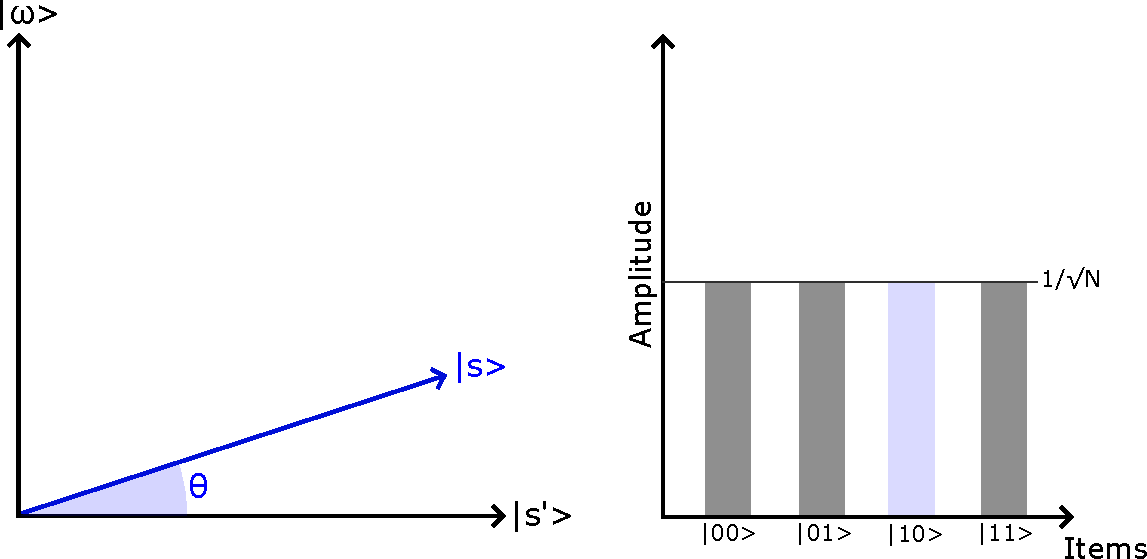
\includegraphics[scale=0.55]{Figures/Grover_Step1.pdf}
    \caption{Amplitude distribution of states after applying a Hadamard gate. The vector $\ket{\omega}$ is our desired state and $\ket{s'}$ is a orthogonal vector. In this way we can write $\ket{s} = \sin{\theta}\ket{\omega} + \cos{\theta}\ket{s'}$.}
    \label{fig:Grover_step1}
\end{figure}
\textbf{(2). Reflection about the state $\ket{s'}$:} Apply an operator $\hat{U}_{\omega}$ defined by
\begin{equation}
     \begin{cases}
       \hat{U}_{\omega}\ket{\omega} = -\ket{\omega} \\
       \hat{U}_{\omega}\ket{i} = \ket{i}, &  \forall \ket{i}\neq \ket{\omega} \\
     \end{cases}
\end{equation}
so the operator can be written as,
\begin{equation}
    \hat{U}_{\omega} = \mathbb{I} - 2\ket{\omega}\bra{\omega}
\end{equation}
Applying the operator to the state $\ket{s}$ yields,
\begin{equation}
    \ket{\psi_{2}} = \hat{U}_{\omega}\ket{s} = \ket{s} -\frac{2}{\sqrt{N}}\ket{\omega} \equiv \ket{\bar{s}}
\end{equation}
\begin{figure}[H]
    \centering
    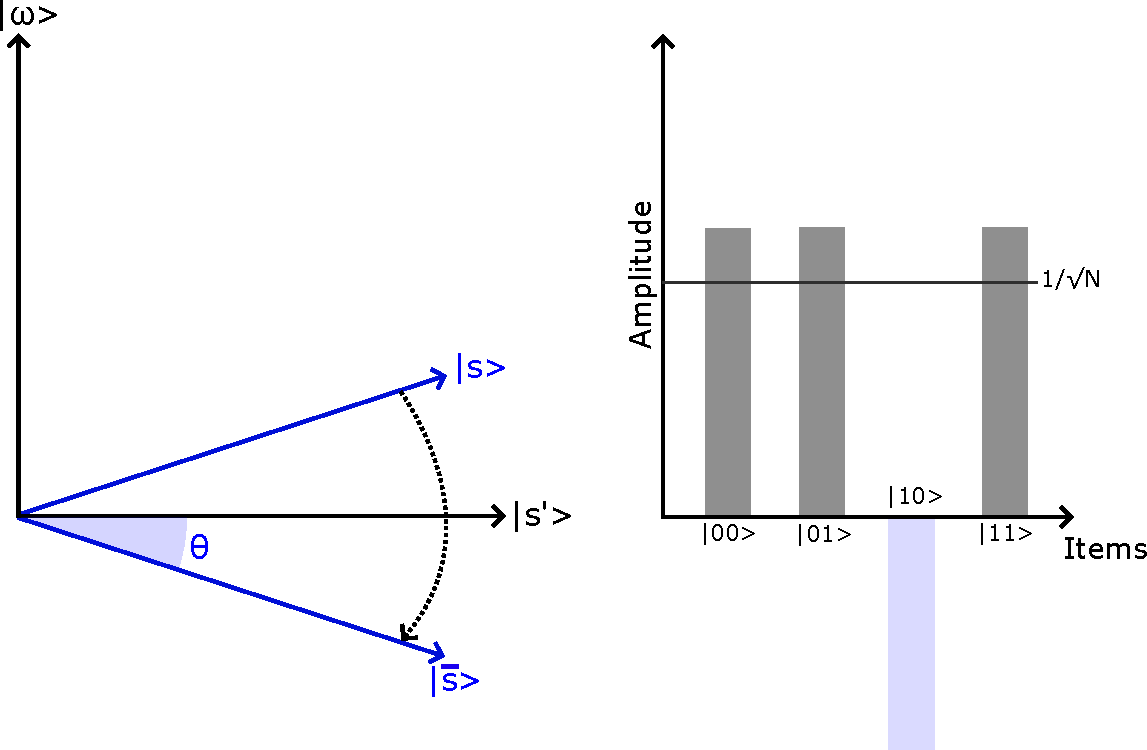
\includegraphics[scale=0.55]{Figures/Grover_Step2.pdf}
    \caption{Amplitude distribution of states after applying a $U_{\omega}$. Notice that we have applied a phase to the state we are looking for. Geometrically this means we have applied a reflection about a state orthonormal to $\ket\omega$.}
    \label{fig:Grover_step2}
\end{figure}
\textbf{(3). Reflection about the state $\ket{s}$:} The operator $\hat{U}_{s}$ is defined as,
\begin{equation}
    \hat{U}_{s} \equiv 2\ket{s}\bra{s} - \mathbb{I}
\end{equation}
Applying the operator to the state of our system yields,
\begin{align*}
    \ket{\psi_{3}} = \hat{U}_{s}\left(\ket{s} -\frac{2}{\sqrt{N}}\ket{\omega}\right) = \left(2\ket{s}\bra{s} - \mathbb{I}\right)\left(\ket{s} - \frac{2}{\sqrt{N}}\ket{\omega}\right) = \frac{N - 4}{N}\ket{s} + \frac{2}{\sqrt{N}}\ket{\omega} \\
    = \frac{1}{N\sqrt{N}} \left[\left(N - 4\right)\sum_{x\neq \omega}\ket{x} + \left(3N-4\right)\ket{\omega}\right] \overset{N=4}{=} \frac{1}{8} \left[0 \cdot \sum_{x\neq \omega}\ket{x} + 8\ket{\omega}\right] = \ket{\omega}
\end{align*}
\begin{figure}[H]
    \centering
    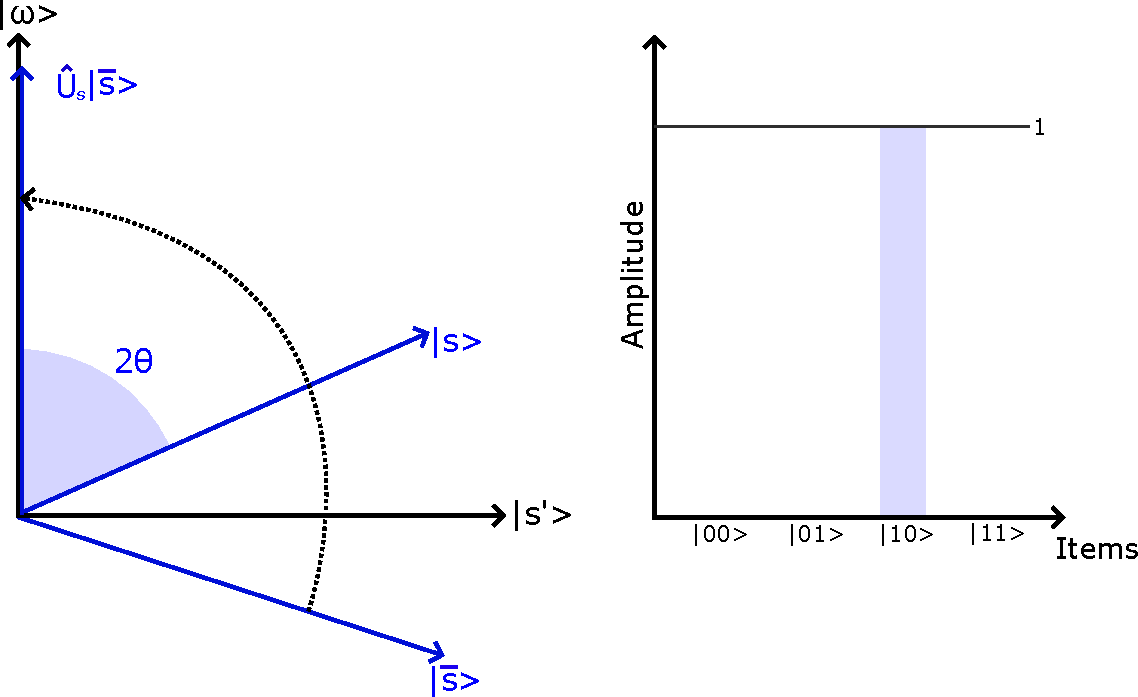
\includegraphics[scale=0.55]{Figures/Grover_Step3.pdf}
    \caption{Amplitude distribution of states after applying $\hat{U}_{s}$. For the case of two qubits, the amplitudes of non-desired states go to zero so we get the desired state $\ket{\omega}$ with a 100\% of probability in an ideal quantum computer. This does not happen if the number of qubits is increased. In that case the amplitudes of non-desired states are reduced compared with the amplitude of the state we are looking for.}
    \label{fig:Grover_step3}
\end{figure}

We have rotated the original state of our system towards the eigenvector $\ket{\omega}$ that represents the item we are looking for in the data-set. The closer\footnote{Notice that the word "close" in this context is referring to the probability of getting the desired state $\ket{\omega}$ when we make a measurement on the system} we want to be to $\ket{\omega}$ the more times we have to repeat \textbf{(2)} and \textbf{(3)}. The quadratic speed up comes from the fact that Grover's algorithm raises the probability amplitude of the item we are looking for by a factor of $\frac{1}{\sqrt{N}}$ .


%Last Comment

